\documentclass[border=6pt]{standalone}
\usepackage[T1]{fontenc}
\usepackage[utf8]{inputenc}
\usepackage[scaled=0.98]{helvet}
\renewcommand{\familydefault}{\sfdefault}
\usepackage{amsmath}
\usepackage{graphicx}
\graphicspath{{../../../../../../exercises_lecturenotes/lecture_notes/kurs100_lektionsnoter/}}
\usepackage{tikz}
\usepackage{pgfplots}
\pgfplotsset{compat=1.18}
\usetikzlibrary{arrows.meta, decorations.pathreplacing, calc, positioning, fit, backgrounds, shapes.geometric}
\usepgfplotslibrary{groupplots,fillbetween}
\definecolor{scanpink}{HTML}{E5006D}
\definecolor{scanteal}{HTML}{00A6A6}
\definecolor{scannavy}{HTML}{243746}
\definecolor{scanlightgray}{HTML}{F1F2F3}
\begin{document}
  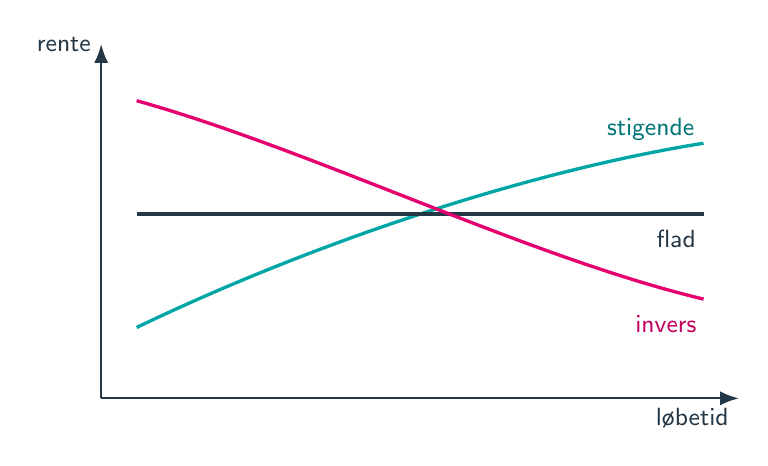
\begin{tikzpicture}[x=0.9cm,y=0.9cm,font=\small]
    \draw[-{Latex[length=2.4mm]},thick,scannavy] (0,0) -- (9,0) node[below left] {løbetid};
    \draw[-{Latex[length=2.4mm]},thick,scannavy] (0,0) -- (0,5) node[left] {rente};
    \draw[very thick,scanteal] (0.5,1) .. controls (3,2.2) and (6,3.2) .. (8.5,3.6);
    \node[scanteal!70!black,anchor=west] at (7.0,3.8) {stigende};
    \draw[very thick,scannavy] (0.5,2.6) -- (8.5,2.6);
    \node[scannavy,anchor=west] at (7.7,2.25) {flad};
    \draw[very thick,scanpink] (0.5,4.2) .. controls (3,3.5) and (6,2.0) .. (8.5,1.4);
    \node[scanpink!85!black,anchor=west] at (7.4,1.05) {invers};
  \end{tikzpicture}
\end{document}
